
% --------------------------------------------------------------- CONFIGURATIONS

%ifdef TWOSIDE
	%\documentclass[a4paper,12pt,final,twoside,openright]{book}
%elif ONESIDE
	\documentclass[a4paper,12pt,final,oneside]{book}
%endif

\usepackage{rapport}



% -------------------------------------------------------------- META: CONSTANTS

\newcommand{\reporttitle}{Digital Image Processing}
\newcommand{\reportauthor}{Thierry~\textsc{Cantenot}}
\newcommand{\reportsubject}{Report}
\newcommand{\topic}{Problem 1: Histogram Equalization}
\newcommand{\HRule}{\rule{\linewidth}{0.5mm}}
\setlength{\parskip}{1ex} % Espace entre les paragraphes

\hypersetup{
	pdftitle={\reporttitle},%
    pdfauthor={\reportauthor},%
    pdfsubject={\reportsubject},%
}

\title{\reporttitle}
\author{\reportauthor}
%\setcounter{tocdepth}{4}


% ------------------------------------------------------------------------- FILE

\begin{document}


    % ------------------------------------------------------------------- HEADER

	\renewcommand{\chaptername}{} %\renewcommand{\thechapter}{}
	\renewcommand{\contentsname}{Summary}

	\pagestyle{empty}
	\pagenumbering{Roman}


    % ------------------------------------------------------------ HEADER: TITLE

	\begin{flushleft}
    \textbf \reportauthor
\end{flushleft}

\vspace{2.0cm}

\begin{center}
	\textsc{\Large \reportsubject}\\[0.3cm]
	\HRule \\[0.4cm]
	{\Huge \bfseries \reporttitle}\\[0.3cm]
	{\LARGE \bfseries «~\topic~»}\\[0.3cm]
	\HRule \\[1cm]

	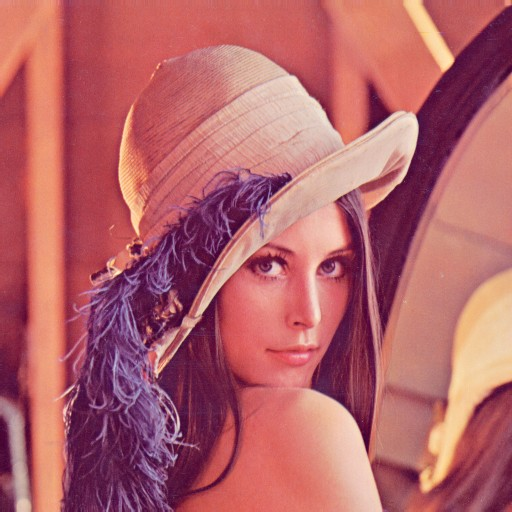
\includegraphics [scale=0.6]{images/lenna.jpg} \\[0.7cm]

	\vfill

    \begin{flushright}
        
\includegraphics[width=40mm]{images/SJTU_Logo.png}
    \end{flushright}

	\footnotesize{2014-2015}
\end{center}


	%ifdef TWOSIDE
		%\cleardoublepage
	%endif

	%\include{title2}

	%ifdef TWOSIDE
		%  \newpage
		%	\null
		%	\vfill
	%endif


    % --------------------------------------------------- HEADER: CONFIGURATIONS

	\sloppy          % Justification moins stricte : des mots ne dépasseront pas des paragraphes

    \frontmatter
		\pagestyle{empty}
		\tableofcontents
		\addtocontents{toc}{\protect\thispagestyle{empty}}

	\mainmatter
	\pagestyle{headings}

	\renewcommand{\thechapter}{\Alph{chapter}}
	\renewcommand{\chaptermark}[1]{\markboth{\MakeUppercase{\chaptername\ \thechapter.\ #1}}{}}
	\renewcommand{\sectionmark}[1]{\markright{\thesection{} #1}}


    % ------------------------------------------------------------------ CONTENT

    \chapter{Problem 1}

\section{Figure 1}

    \subsection{Histogram}

    \begin{figure}[h]
        \centering
        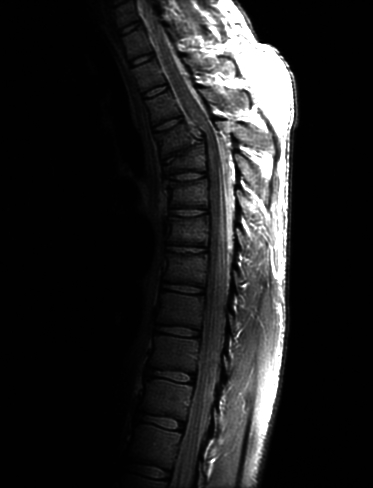
\includegraphics[width=\linewidth]{./images/Fig1.jpg}
        \caption{Fig1.jpg}
        \label{diagram:fig1}
    \end{figure}

    \begin{figure}[h]
        \centering
        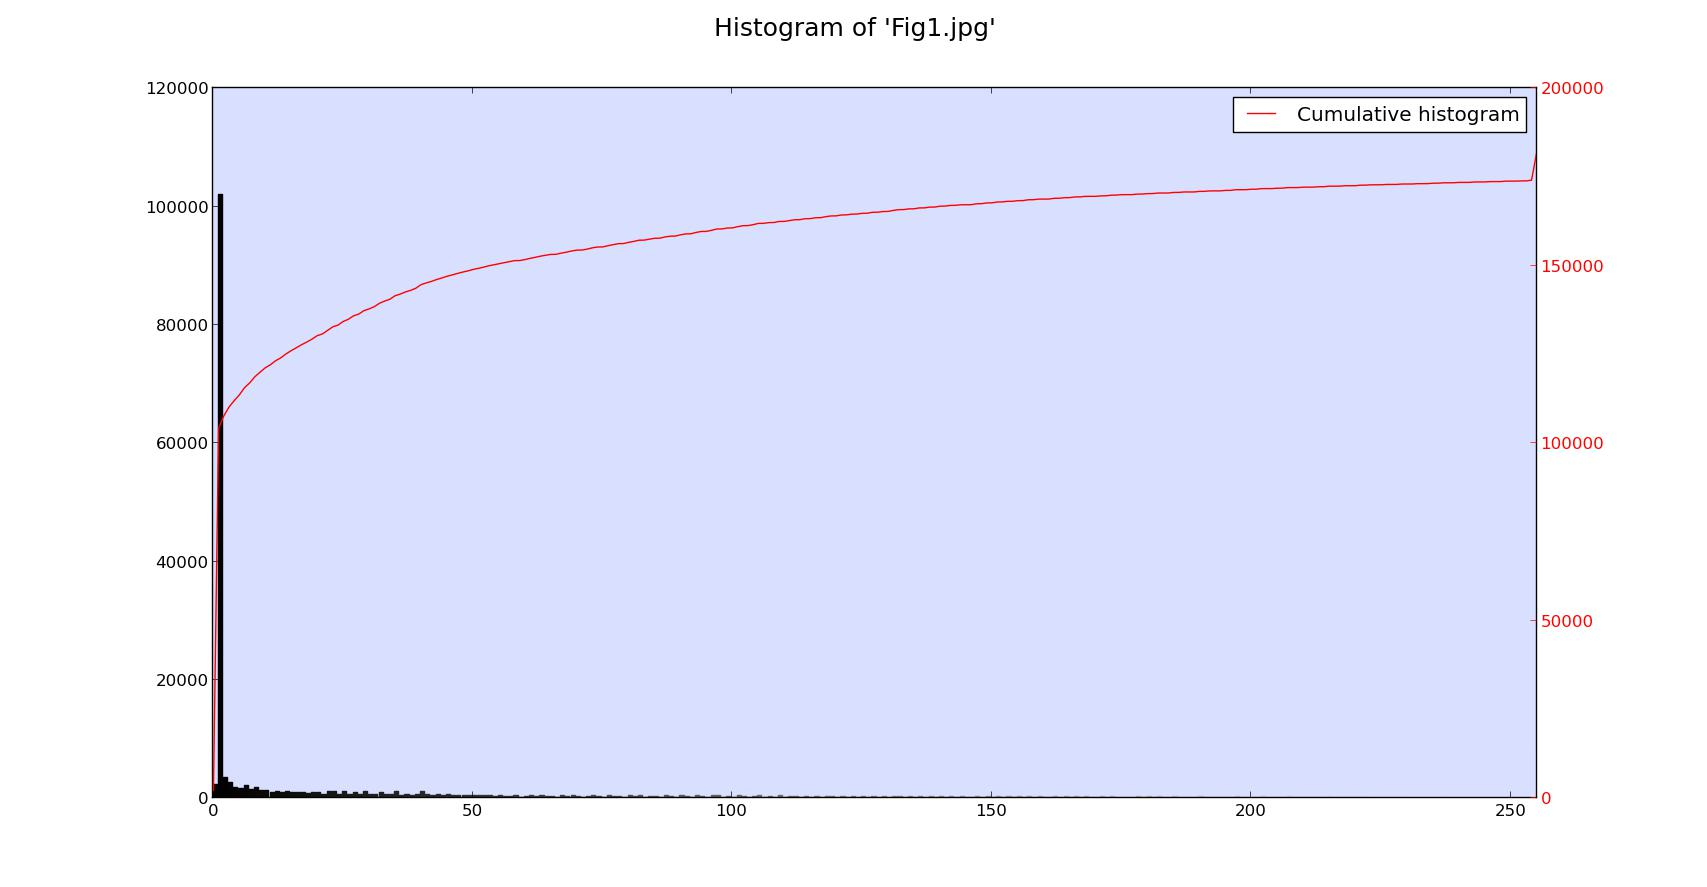
\includegraphics[width=\linewidth]{./images/Histogram_Fig1.jpg}
        \caption{Histogram of "Fig1.jpg"}
        \label{diagram:hist_fig1}
    \end{figure}

    \subsection{Histogram equalization}

    \begin{figure}[h]
        \centering
        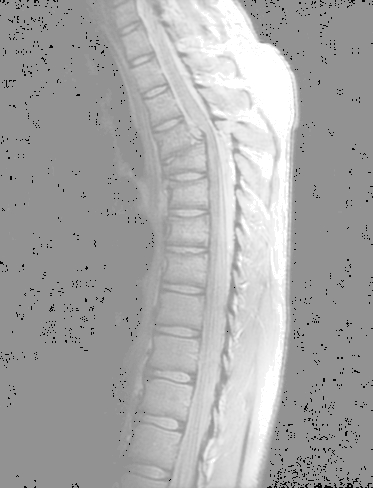
\includegraphics[width=\linewidth]{./images/Enhanced_Fig1.jpg}
        \caption{Enhanced Fig1.jpg}
        \label{diagram:enhanced_fig1}
    \end{figure}

    \begin{figure}[h]
        \centering
        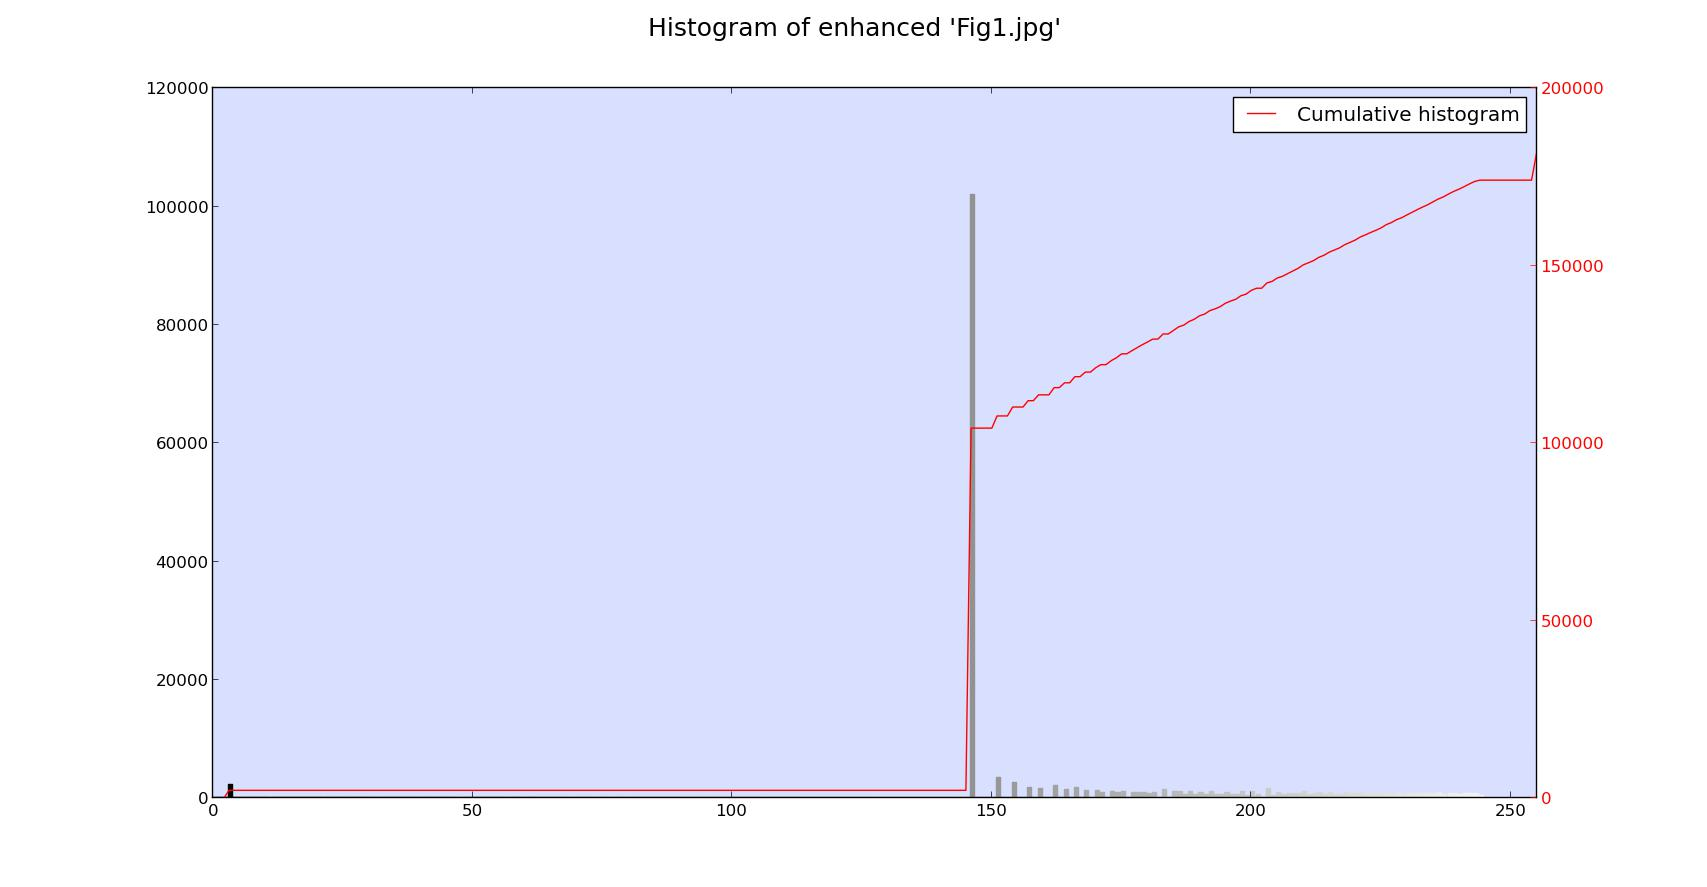
\includegraphics[width=\linewidth]{./images/Equalized_Histogram_Fig1.jpg}
        \caption{Equalized histogram of "Fig1.jpg"}
        \label{diagram:equal_hist_fig1}
    \end{figure}


\section{Figure 2}

    \subsection{Histogram}

    \begin{figure}[h]
        \centering
        
\includegraphics[width=\linewidth]{./images/Fig2.jpg}
        \caption{Fig1.jpg}
        \label{diagram:fig1}
    \end{figure}

    \begin{figure}[h]
        \centering
        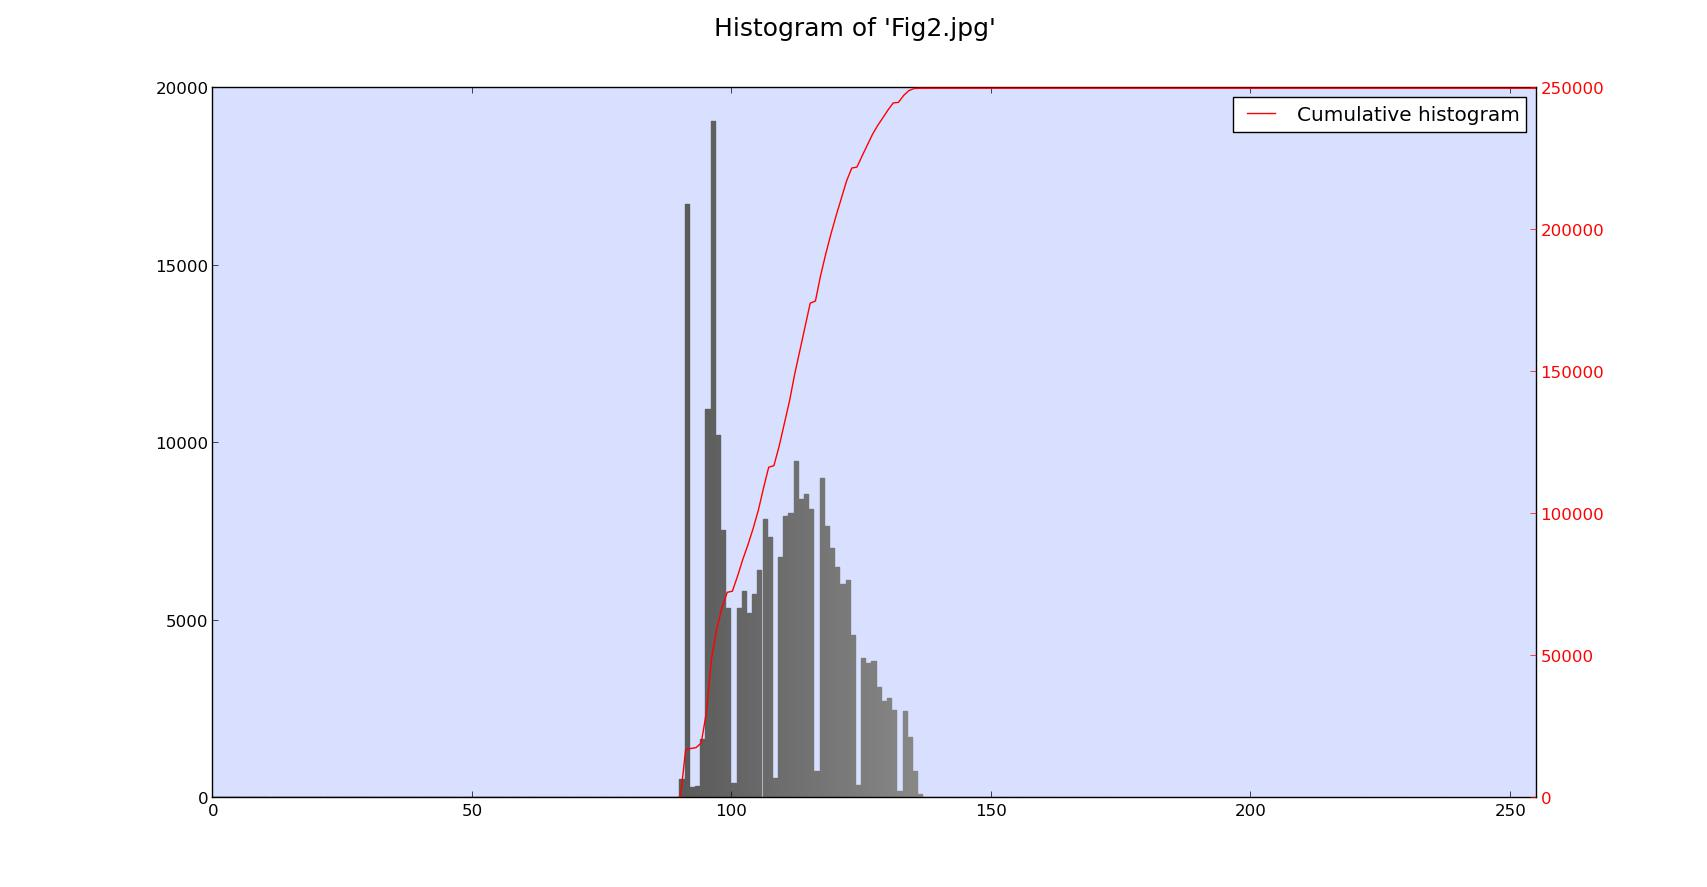
\includegraphics[width=\linewidth]{./images/Histogram_Fig2.jpg}
        \caption{Histogram of "Fig1.jpg"}
        \label{diagram:hist_fig2}
    \end{figure}

    \subsection{Histogram equalization}

    \begin{figure}[h]
        \centering
        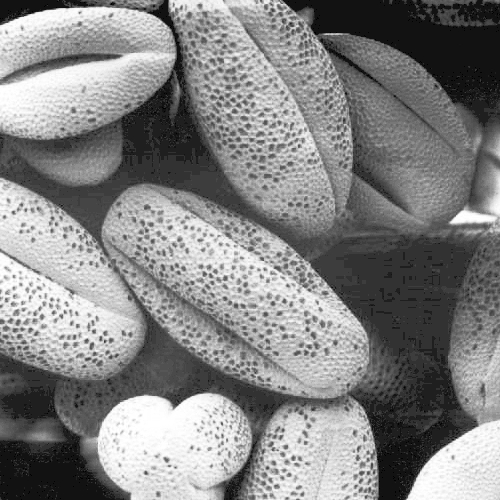
\includegraphics[width=\linewidth]{./images/Enhanced_Fig2.jpg}
        \caption{Enhanced "Fig2.jpg"}
        \label{diagram:enhanced_fig2}
    \end{figure}

    \begin{figure}[h]
        \centering
        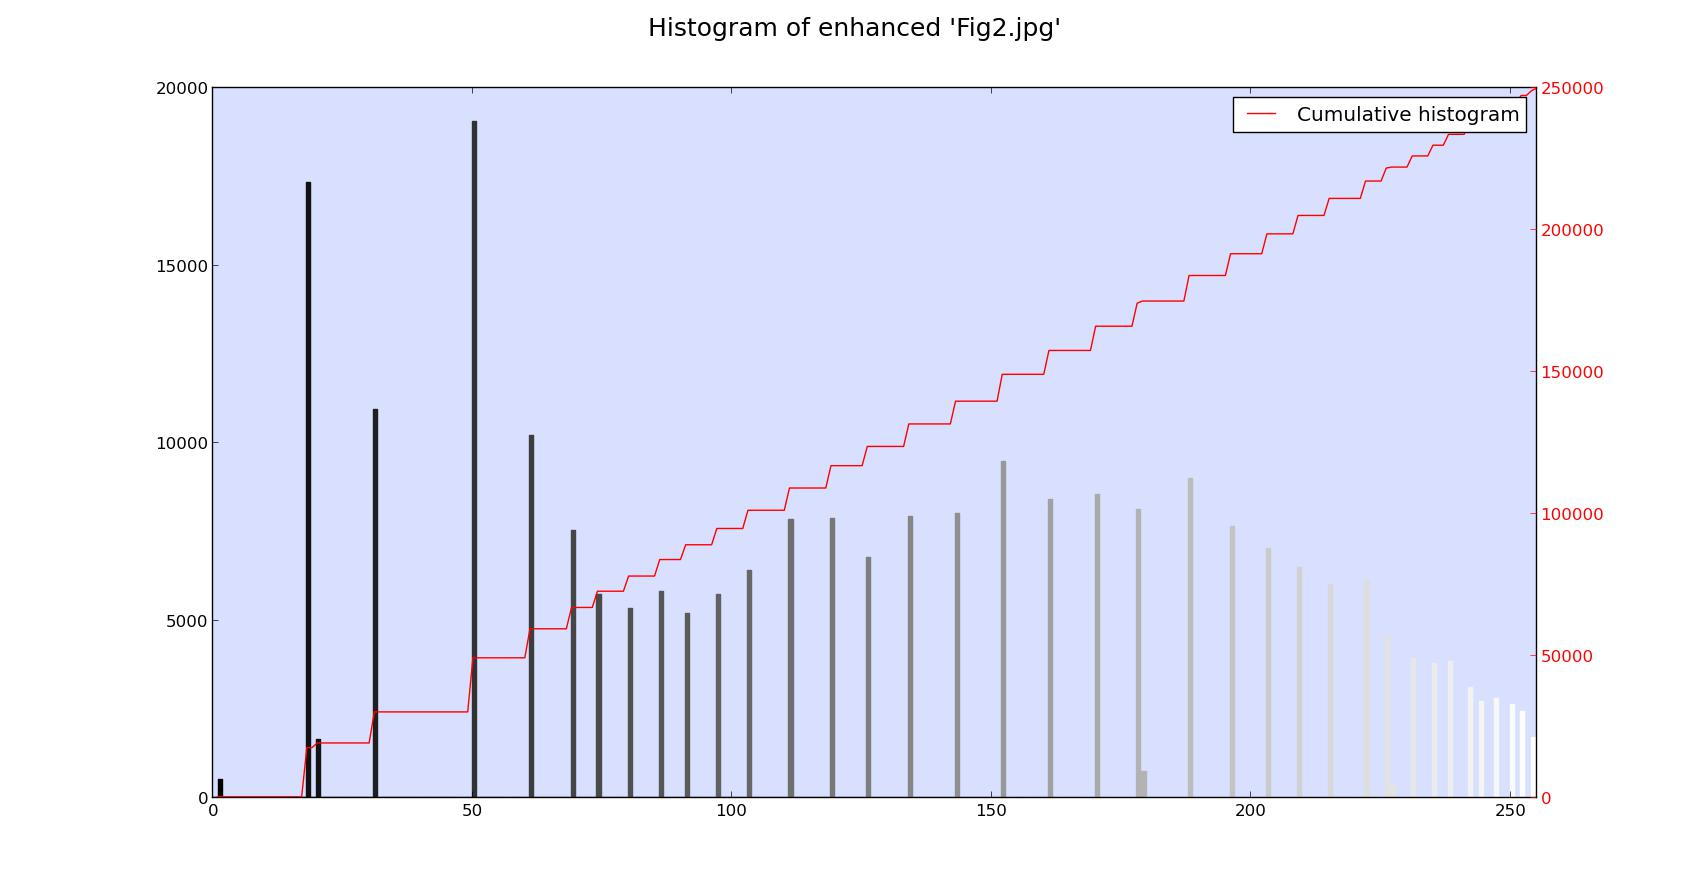
\includegraphics[width=\linewidth]{./images/Equalized_Histogram_Fig2.jpg}
        \caption{Equalized histogram of "Fig2.jpg"}
        \label{diagram:equal_hist_fig2}
    \end{figure}



    % ------------------------------------------------------------------- FOOTER
\end{document}
